
\documentclass[12pt,journal,compsoc]{IEEEtran}
\usepackage[spanish]{babel}
\usepackage{array}
\usepackage{graphicx}
\usepackage{diagbox}
\usepackage{float}
\usepackage[utf8]{inputenc}
\newcommand\MYhyperrefoptions{bookmarks=true,bookmarksnumbered=true,
pdfpagemode={UseOutlines},plainpages=false,pdfpagelabels=true,
colorlinks=true,linkcolor={black},citecolor={black},urlcolor={black},
pdftitle={Relación entre la legibilidad de una serie de libros y sus respectivas calificaciones},
pdfsubject={Neurociencia},
pdfauthor={Sabrina Izcovich, Roberto Rama, Gustavo Juantorena},
pdfkeywords={Neurociencia, Vocabulario, Libro, Métricas, Legibilidad}}

\begin{document}
\title{Relación entre la legibilidad de libros y sus respectivas calificaciones}

\author{Gustavo~Juantorena~~~~~~
        Roberto~Rama~~~~~~
        Sabrina~Izcovich\\
        \textit{Facultad de Ciencias Exactas, UBA}}


\IEEEtitleabstractindextext{

\begin{abstract}Desde tiempos inmemoriables las personas han expresado variados gustos y opiniones sobre distintos tópicos, siendo la literatura uno de los más discutidos. Los fundamentos de las opiniones pueden ser muy variados e incluso difusos para los dueños de las mismas. A pesar de esto, las personas son capaces de asignar un puntaje numérico comparativo a una obra, que dado un número grande de puntajes tiende a converger a un número, evidenciando asi una especie de acuerdo en el gusto general. Estos sistemas de puntajes son normalmente utilizados por las tiendas online, como una forma de guía confiable para otros clientes, pero además son una fuente de información muy interesante. En el presente trabajo práctico ponemos a prueba la hipótesis de que la forma de escritura de un libro influye en la recepción del mismo por la población, siendo libros mas legibles mejor valorados. Demostramos la validez de esta hipótesis analizando distintas métricas de legibilidad clásicas en una fracción de los libros de la base de datos de Amazon, asegurando cierta homogeneidad en la selección de los mismos utilizando sus categorías.
\end{abstract}

% cita en ``puntaje numerico comparativo a una obra''

\begin{IEEEkeywords}
Neurociencia, Métricas, Legibilidad, Libros, Reseñas.
\end{IEEEkeywords}}

\maketitle
\IEEEdisplaynontitleabstractindextext
\IEEEpeerreviewmaketitle

\section{Introducción}
\IEEEPARstart{E}{n la actualidad,} el avance de la tecnología permite compartir experiencias de distinta índole entre sus usuarios. Por ejemplo, el intercambio de críticas y comentarios sobre diferentes productos, que pueden ocasionar un aumento o disminución de sus respectivas ventas. Es por esto que conocer los motivos de los usuarios a la hora de calificar resulta útil cuando se desea estudiar el mercado. En este trabajo, analizamos libros en base al nivel de legibilidad de los mismos con el fin de encontrar relaciones entre éste y la valoración que reciben. 

A continuación, se presenta un estudio cuyo fin es encontrar una relación entre las calificaciones de libros halladas en el sitio de compraventa $Amazon$\footnote{www.amazon.com}, y el grado de legibilidad de los mismos. Para ello, recompilamos una amplia variedad de libros de distintos autores, géneros y formatos, junto con la información de las calificaciones asignadas por sus lectores. Por otro lado, debimos considerar una forma de medir el grado de legibilidad, para lo que elegimos el Readability test\footnote{http://shop.niace.org.uk/media/catalog/product/R/e/Readability.pdf}, que consiste en una serie de fórmulas para evaluar la legibilidad de un texto, ya sea contando sílabas, palabras o frases.

El proyecto consiste en poder predecir futuras calificaciones de acuerdo a la comprensión del libro en cuestión, partiendo de la hipótesis de que, a partir de ciertas métricas, puede analizarse su contenido y luego relacionarse significativamente con el puntaje otorgado por los lectores\footnote{http://snap.stanford.edu/data/amazon-meta.html}.

En primer lugar, se explicará el proceso realizado a lo largo del estudio y las herramientas empleadas detalladamente, incluyendo el criterio de clasificación de los libros y sus puntajes, como también las métricas empleadas. Luego, se expondrán los resultados empíricos obtenidos por categoría y la correlación entre éstos. Más tarde, presentaremos un análisis estadístico de los resultados medidos que nos permitirán, finalmente, extraer conclusiones.

\section{Trabajos relacionados}
Con el fin de orientar nuestra investigación, revisamos distintos estudios realizados y ciertos documentos correspondientes al área. En uno de los más relevantes (\textit{Graesser, A. C. et al., 2004} \cite{graesser}), los autores utilizaron el software \textit{Coh-metrix} para clasificar los textos según la dificultad de lectura que presentan (avanzado, intermedio, principiante). Para evaluar el constructo legibilidad (``readibility'') se implementaron dos fórmulas (``Lesch Reading Ease score'' y ``Flesch Kincaid Grade Level''), herramientas tradicionales para evaluar la complejidad de textos en inglés.\\
Por otro lado, a partir de otro trabajo del mismo grupo (\textit{Crossley, S. A., et al., 2011} \cite{crossley}), pudimos orientarnos en lo que respecta el procesamiento automático de textos con el fin de obtener algún parámetro numérico sobre su contenido. En el mismo, los autores comparan dos herramientas (``Coh-Metrix Second Language (L2) Reading Index'' versus métodos tradicionales como los del trabajo anteriormente citado) para medir coherencia, legibilidad y otros constructos en forma sencilla en un gran corpus de texto.\\
Finalmente, el trabajo presentado durante las clases teóricas (\textit{Diuk, C. G., et. al., 2012} \cite{diuk}), resultó de gran utilidad como inspiración sobre la potencialidad del análisis de grandes repositorios de datos con el fin de hacer predicciones. En el mismo, se utilizaron  textos de distintas épocas en orden cronológico con el fin de probar si el constructo introspección creció o disminuyó a lo largo de los años.

\section{Métodos}

En lo que sigue, se presentan los métodos utilizados para el ánalisis mencionado.

\subsection{Métricas utilizadas}
\subsubsection{LIX}

\textbf{LIX}\footnote{http://www.readabilityformulas.com/the-LIX-readability-formula.php} es una medida de legibilidad para calcular la dificultad de lectura de un texto desarrollada por Carl-Hugo Björnsson:

$$LIX\ =\ \frac{palabras}{periodos} + \ 100 \cdot \frac{palabras\ largas}{palabras}$$

En donde se define como períodos dos puntos o primera mayúscula\\

\subsubsection{ARI}
El índice de legibilidad automatizado (\textbf{ARI}) fue diseñado para medir la comprensividad de un texto. Su fórmula para calcular la legibilidad automática se da en la siguiente relación:

$$ARI = 4.71\cdot \frac{caracteres}{palabras}+0.5\cdot \frac{palabras}{frases} - 21.43$$

donde \textit{caracteres} corresponde a la cantidad de letras y números, \textit{palabras} es la cantidad de espacios y \textit{frases} la cantidad de frases.

\subsubsection{Flesch reading ease}

La fórmula de \textbf{Flesch reading ease score test} es la siguiente:
$$FRE = 206.835 - 1.015\cdot \frac{palabras}{frases} - 84.6\cdot \frac{silabas}{palabras}$$

\subsubsection{Coleman-Liau index}
Test de legibilidad diseñado por Meri Coleman y T. L. Liau. Se lo calcula de la siguiente forma: 
$$CLI = 5.88 \cdot \frac{letras}{palabras} - 29.6 \cdot \frac{frases}{palabras} - 15.8$$

\subsubsection{SMOG}
El grado \textbf{SMOG} (Medida simple de Gobbledygook) es una medida de legibilidad que estima los años de educación necesarios para entender un texto. Para calcularlo, se debe contar una serie de frases (al menos 30) y contar las polisílabas (palabras de tres o más sílabas) que posee cada una de ellas. Se calcula usando 

$$SMOG = 1.0430\cdot \sqrt{polisilabas \cdot \frac{30}{frases}} + 3.1291$$


\subsubsection{Resultado con Harry Potter}
\begin{tabular}{| l | l | l | l | l | l | l |}
\hline
\diagbox[width=10em]{Libro}{Métrica} & ARI & Coleman-Liau & Flesch Reading Ease & LIX & SMOG & Dale-Chall\\
\hline
HP1 & 4.48 & 6.37 & 92.58 & 27.00 & 7.18 & 8.77\\
\hline
HP2 & 5.41 & 7.19 & 87.88 & 29.74 & 7.74 & 9.17\\
\hline
HP3 & 5.19 & 7.26 & 87.37 & 29.61 & 7.64 & 9.14\\
\hline
HP4 & 6.01 & 7.52 & 85.17 & 30.80 & 8.15 & 9.16\\
\hline
HP5 & 6.67 & 7.82 & 83.34 & 32.84 & 8.49 & 9.22\\
\hline
HP6 & 6.48 & 7.76 & 82.55 & 32.30 & 8.60 & 9.13\\
\hline
HP7 & 5.87 & 7.47 & 85.47 & 30.82 & 8.13 & 8.97\\
\hline
\end{tabular}

Con el fin de comprobar la correctitud de dichas métricas, evaluamos el resultado de evaluar la saga \textit{Harry Potter}\footnote{http://cor.to/harrypotter}, que presenta (según su autora \footnote{http://www.jkrowling.com/}) una dificultad creciente en el vocabulario de sus títulos.\\

\subsection{Libros analizados}
En lo que sigue, se explican las consideraciones que tuvimos en cuenta a la hora de seleccionar los libros a analizar. En primer lugar, estudiamos el conjunto de categorías presentadas por Amazon y las posibles reseñas (utilizando la escala del 0 al 5, saltando de a 0.5). Luego, decidimos dividir las categorías en cuatro clusters (numerados  del 1 al 4), y descargar 15 libros de cada reseña y cada cluster. Dado que no encontramos libros con reseñas del 0 al 1.5, y la cantidad de libros calificados con 1.5 era escasa, insertamos los libros de 1.5 a 2.5 en un mismo puntaje, y para el resto se usó la descripción anterior.\\

En primer lugar, descargamos la base de datos \textit{Amazon product co-purchasing network metadata}\footnote{http://snap.stanford.edu/data/amazon-meta.html} en donde se detallan productos (dentro de los cuales 393.561 son libros), ranking de ventas, categoría de los mismos y reseñas en el sitio de Amazon.com. Al analizarla, nos encontramos con que, además de que la mayoría de los libros se encontraba en diversas categorías a la vez, éstas aparecen acompañadas de todos los subconjuntos de la jerarquía a la que pertenecen. Por ejemplo, la categoría ``Drama'' aparece junto con ``Books'', ``Subjects'', ``Literature \& Fiction'', por lo que ciertos libros terminan perteneciendo a 16 o más categorías. Por otro lado, nos encontramos con que gran parte de los productos se encontraban repetidos, ya sea por poseer distintas ediciones, distintos formatos (tapa blanda/tapa dura, con audio, con dibujos, etc) o por estar clasificados de forma diferente. 
%Podriamos mostrar un histograma en donde se vea la distribucion de los puntajes en relacion a la cantidad de libros y otro con la cantidad de scores (para que se vea que hay pocos libros con muchos scores y muchos con pocos). Podemos explicar que la obtencion de los libros en si se dificulto un poco para los puntajes bajos y en donde la cantidad de scores era menor a 100.
Luego, procedimos a descargar los libros, tarea que resultó altamente dificultosa para las obras poco populares o de bajo puntaje dada la falta de interés a digitalizarlos. La selección de los mismos se realizó como se explica a continuación.

\subsubsection{Filtrado de los libros} Aca podemos explicar como hicimos para ordenar los libros de la lista para seleccionar a mano y como funciona el script (getBooks.py)
Para lograr resultados significativos, analizamos 156 libros que clasificamos de acuerdo a las categorías con requerimientos de palabras clave provistas por Amazon.com\footnote{http://cor.to/categories}. Para lograr mayor organización y homogeneidad en nuestro análisis, decidimos unificarlas en los siguientes clusters:
\begin{itemize}
\item \textbf{Cluster Nº1:} Science Fiction and Fantasy, Classics, Fantasy, World Literature
\item \textbf{Cluster Nº2:} Religion and Spirituality, Fiction, Health Mind and Body, Self-Help
\item \textbf{Cluster Nº3:} Mystery and Thrillers, Thrillers, Biographies and Memoirs, Suspense, Nonfiction, History, Politics, Social Science
\item \textbf{Cluster Nº4:} Other categories
\end{itemize}
De este modo, conseguimos una cantidad uniforme de libros por cluster.

\section{Experimentos y Resultados}

\subsection{Eliminacion parcial del sesgo}

Dado que libros de distintas categorias pueden presentar distinto vocabulario, los resultados pueden verse sesgados si utilizamos para el analisis muchos libros de una tematica parecida. Para asegurarnos una homogeneidad conformamos 4 conjuntos o clusters distintos de libros, en donde cada cluster esta compuesto por categorias distintas, de forma tal de asegurarnos un analisis con libros de distintas categorias, distinto vocabulario y enfocados para distinto publico.

El dataset crudo presenta el problema de que las categorias no conforman conjuntos disjuntos y ademas hay cierta jerarquia presente en las mismas. Para eliminar las categorias de los niveles inferiores de la jerarquia filtramos aquellas que aparecian 50 veces o menos, resultando en una lista de 129 categorias principales. De esta lista eliminamos categorias demasiado generales o poco descriptivas como ``Bargain Books'', ``Authors A-Z'', ``Age 3-5'', entre otras; llegando a una lista final de 113 categorias.

% TODO: Agregamos grafo de jerarquia?

Habiendo confeccionado esta lista realizamos una codificacion de la base de datos en donde cada libro puede ser descripto como una tira de ceros y unos, en donde cada cero o uno indica la pertenencia a una categoria. Utilizando Weka ejecutamos un algoritmo de clusterizacion llamado expectation maximization con 10 folds y 8 clusters. Si bien nuestro objetivo original era obtener 4 clusters, si especificabamos esta cantidad uno de los clusters agrupaba demasiados libros, ya que el algoritmo agrupa todos aquellos que no puede terminar de clasificar (por el limite asignado) en uno solo.

Como en todos los clusters existen libros que contienen categorias de otros clusters, formar clusters totalmente disjuntos en las categorias es imposible. Sin embargo podemos intentar formarlos minimizando la cantidad de libros que comparten categorias con otros clusters. Probamos distintas maneras de agrupar los clusters y finalmente la composicion quedo definida de la siguente manera:

~

\begin{itemize}
 \item Cluster N1: Science Fiction And Fantasy, Fantasy, Science Fiction, Classics, World Literature
 \item Cluster N2: Religion And Spirituality, Health Mind And Body, Fiction, Self-Help
 \item Cluster N3: Mystery And Thrillers, Thrillers, Suspense, Biographies And Memoirs, Nonfiction, History, Politics, Social Sciences
 \item Cluster N4: El resto
\end{itemize}
% TODO: Falta pie de cuadro

~

De esta manera solo un 20\% de los libros comparte categorias de 2 clusters distintos. Un analisis rapido de las cantidades contenidas en cada cluster arroja nos dice que si bien la division esta lejos de ser perfecta en lo que respecta a cantidades nominales, nos da margen suficiente para analizar libros de distintos puntajes y clusters.

~

\begin{table}
 \centering
  \begin{tabular}{| l | l | l | l | l |}
  \hline
  \diagbox[width=10em]{Puntaje}{Cluster} & 1 & 2 & 3 & 4 \\
  \hline
  1.5  & 4     & 2    & 19   & 5    \\
  \hline
  2    & 6     & 4    & 35   & 27   \\
  \hline
  2.5  & 36    & 33   & 103  & 66   \\
  \hline
  3    & 107   & 139  & 414  & 237  \\
  \hline
  3.5  & 450   & 390  & 855  & 733  \\
  \hline
  4    & 1394  & 863  & 1483 & 1366 \\
  \hline
  4.5  & 1801  & 1661 & 1610 & 1800 \\
  \hline
  5    & 232   & 355  & 230  & 322  \\
  \hline
    Total & 4030  & 3447 & 4749 & 4556 \\
    \hline
  \end{tabular}
\end{table}

\subsection{Análisis de Datos} 
analisis de datos de amazon y de los libros que bajamos
%Ademas hay que explicar cuantos libros agarramos de cada categoria principal y porque decidimos dejar los que tenian menos de 100 reviews fuera (basicamente, es por la convergencia del promedio de una muestra). \subsection{Resultados de las métricas} Podemos mostrar graficos de histogramas combinados, uno para los resultados de los libros ``Buenos'' y otros para los ``Malos'' de las 3 metricas: cantidad de palabras simple english, cantidad de vocabulario simple english y cantidad de repeticiones. Podemos decir que en un principio decidimos eliminar la cantidad de palabras como una metrica ya que da siempre entre 40\% y 50\% para todos los libros.\\

\subsection{Análisis de Resultados}

\begin{minipage}{\linewidth}
  \centering
  \begin{minipage}{0.25\linewidth}
      \begin{figure}[H]
          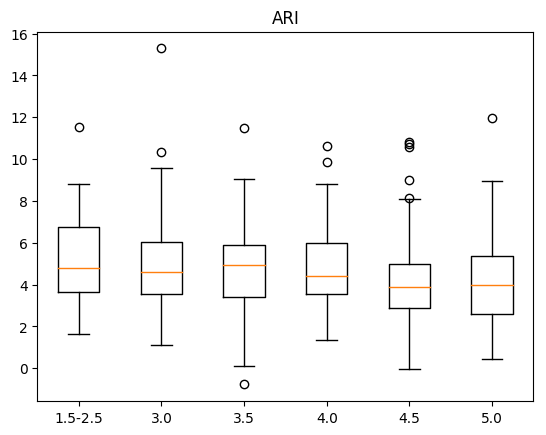
\includegraphics[width=2.3in]{../unigrams/scripts/boxplots/not-normalized-ARI.png}
          \caption{ARI}
      \end{figure}
  \end{minipage}
  \hspace{0.05\linewidth}
  \begin{minipage}{0.25\linewidth}
      \begin{figure}[H]
          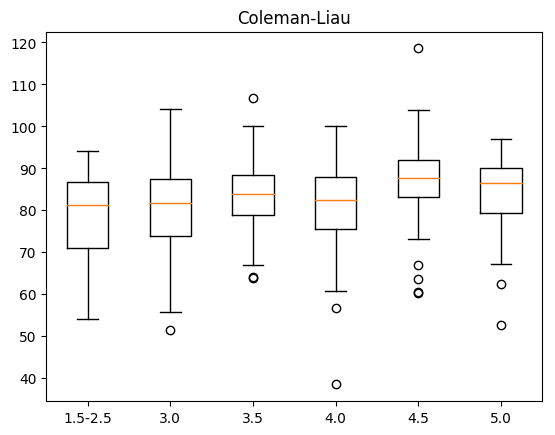
\includegraphics[width=2.3in]{../unigrams/scripts/boxplots/not-normalized-Coleman-Liau.png}
          \caption{Coleman-Liau}
      \end{figure}
  \end{minipage}
  \hspace{0.05\linewidth}
  \begin{minipage}{0.25\linewidth}
      \begin{figure}[H]
          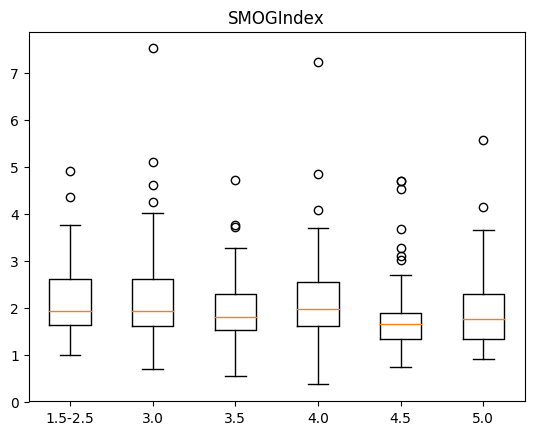
\includegraphics[width=2.3in]{../unigrams/scripts/boxplots/not-normalized-SMOGIndex.png}
          \caption{SMOGIndex}
      \end{figure}
  \end{minipage}
\end{minipage}

\begin{minipage}{\linewidth}
  \centering
  \begin{minipage}{0.25\linewidth}
      \begin{figure}[H]
          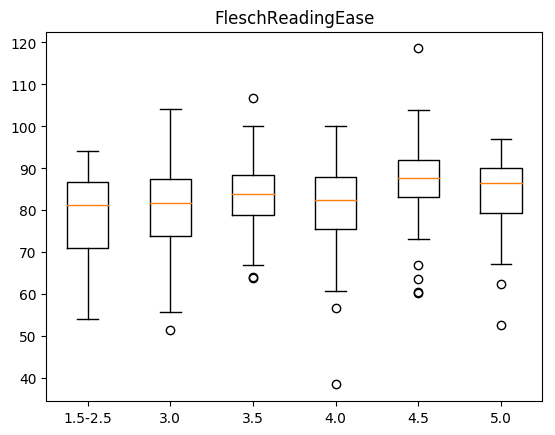
\includegraphics[width=2.3in]{../unigrams/scripts/boxplots/not-normalized-FleschReadingEase.png}
          \caption{FleschReadingEase}
      \end{figure}
  \end{minipage}
  \hspace{0.05\linewidth}
  \begin{minipage}{0.25\linewidth}
      \begin{figure}[H]
          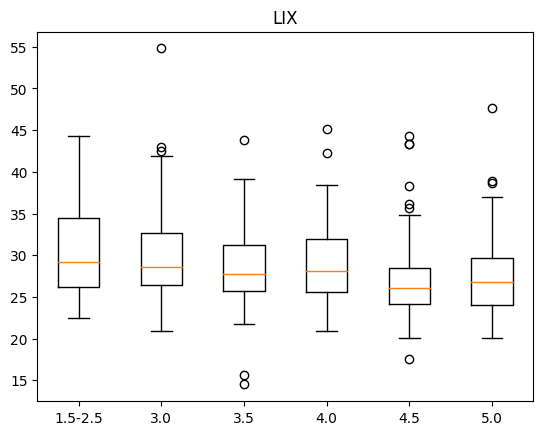
\includegraphics[width=2.3in]{../unigrams/scripts/boxplots/not-normalized-LIX.png}
          \caption{LIX}
      \end{figure}
  \end{minipage}
  \hspace{0.05\linewidth}
  \begin{minipage}{0.25\linewidth}
      \begin{figure}[H]
          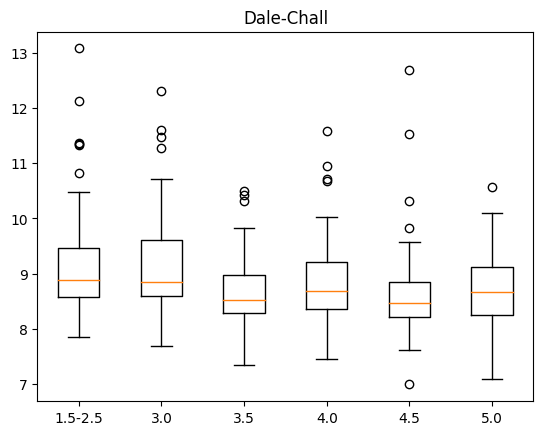
\includegraphics[width=2.3in]{../unigrams/scripts/boxplots/not-normalized-Dale-Chall.png}
          \caption{Dale-Chall}
      \end{figure}
  \end{minipage}
\end{minipage}

\subsection{Análisis de los Resultados del Test de Hipótesis}

Para plantear los Test de Hipótesis correspondientes utilizamos la función $ks\_2samp$\footnote{https://docs.scipy.org/doc/scipy-0.15.1/reference/generated/scipy.stats.ks\_2samp.html} de la librería scipy. El mismo computa el estadístico Kolmogorov-Smirnov en dos muestras. Éste es un test para la hipótesis nula de que dos muestras independientes se consiguen de la misma distribución continua.\\

Luego, dados dos arreglos \textbf{a} y \textbf{b} se obtienen \textbf{D} (o estadístico KS) y el p-valor. Si el estadístico KS es pequeño o el p-valor grande, no podemos rechazar la hipótesis de que las dos muestras son de la misma distribución.\\

% TODO: Falta la cita sobre la necesidad de estas condiciones

La Hipótesis nula es rechazada con nivel $\alpha$ si $$D > c(\alpha) \sqrt{\frac{n_1+n_2}{n_1\cdot n_2}}$$ donde $n_1$ y $n_2$ son los tamaños de las muestras a comparar. El valor de $c(\alpha)$ se define como:
$$c(\alpha) = \sqrt{1/2\ log(\alpha/2)}$$

Los resultados obtenidos con un nivel de significancia de 0.001 para las métricas analizadas fueron los siguientes:\\

\begin{tabular}{ | l | l | l | l | }
\hline
Métrica & P-valor & D & Decisión sobre la Hipótesis nula\\
\hline
ARI & 1.9e-2 & 1.929e-2 & \textbf{NO rechazada} (1.9e-2 $<$ 0.001 y 2.5e-2 $<$ 1.929e-2)\\
\hline
LIX & 1.684e-3 & 2.378e-1 & \textbf{NO rechazada} (1.684e-3 $<$ 1e-3 y 2.5e-1 $<$ 2.378e-1)\\
\hline
Coleman-Liau & 5.97e-4 & 2.546e-1 & \textbf{Rechazada} (5.97e-4 $<$ 1e-3 y 2.5e-1 $<$ 2.546e-1)\\
\hline
FleschReadingEase & 9.126e-05 & 2.82e-1 & \textbf{Rechazada} (9.126e-05 $<$ 1e-3 y 2.5e-1 $<$ 2.82e-1)\\
\hline
Dale-Chall & 2.52e-05 & 3e-1 & \textbf{Rechazada} (2.52e-05 $<$ 1e-3 y 2.5e-1 $<$ 3e-1)\\
\hline
SMOGIndex & 8.01e-06 & 3.15e-1 & \textbf{Rechazada} (8.01e-06 $<$ 0.001 y 2.5e-1 $<$ 3.15e-1)\\
\hline
\end{tabular}


\section{Conclusiones y trabajo futuro} Por lo que vi vamos a tener que decir que obtuvimos resultados significativos pero los numeros estan demasiado cercanos como para utilizar la metrica como criterio. Explicar que otras metricas se nos ocurren para lo cual podria funcionar. Por ejemplo, a mi se me ocurre que una metrica mutli-variable con elementos de procesamiento de lenguaje natural podria dar mejores resultados, es decir metricas que describan mejor la forma en que el libro esta escrito.\\

%\begin{figure}[!t]
%\centering
%\includegraphics[width=2.5in]{myfigure}
% where an .eps filename suffix will be assumed under latex, 
% and a .pdf suffix will be assumed for pdflatex; or what has been declared
% via \DeclareGraphicsExtensions.
%\caption{Simulation Results.}
%\label{fig_sim}
%\end{figure}

% An example of a double column floating figure using two subfigures.
% (The subfig.sty package must be loaded for this to work.)
% The subfigure \label commands are set within each subfloat command,
% and the \label for the overall figure must come after \caption.
% \hfil is used as a separator to get equal spacing.
% Watch out that the combined width of all the subfigures on a 
% line do not exceed the text width or a line break will occur.
%
%\begin{figure*}[!t]
%\centering
%\subfloat[Case I]{\includegraphics[width=2.5in]{box}%
%\label{fig_first_case}}
%\hfil
%\subfloat[Case II]{\includegraphics[width=2.5in]{box}%
%\label{fig_second_case}}
%\caption{Simulation results.}
%\label{fig_sim}
%\end{figure*}


% An example of a floating table. Note that, for IEEE style tables, the 
% \caption command should come BEFORE the table. Table text will default to
% \footnotesize as IEEE normally uses this smaller font for tables.
% The \label must come after \caption as always.
%
%\begin{table}[!t]
%% increase table row spacing, adjust to taste
%\renewcommand{\arraystretch}{1.3}
% if using array.sty, it might be a good idea to tweak the value of
% \extrarowheight as needed to properly center the text within the cells
%\caption{An Example of a Table}
%\label{table_example}
%\centering
%% Some packages, such as MDW tools, offer better commands for making tables
%% than the plain LaTeX2e tabular which is used here.
%\begin{tabular}{|c||c|}
%\hline
%One & Two\\
%\hline
%Three & Four\\
%\hline
%\end{tabular}
%\end{table}


%\ifCLASSOPTIONcaptionsoff
%  \newpage
%\fi

\begin{thebibliography}{1}

\bibitem{graesser}
Graesser,~A.~C.,~McNamara,~D.~S.,~Louwerse,~M.~M., \& Cai,~Z. (2004). ``Coh-Metrix: Analysis of text on cohesion and language.''\footnote{http://cor.to/graesser} \hskip 1em plus
  0.5em minus 0.4em\relax \emph{Behavior Research Methods,Instruments, \& Computers}, 36(2), 193-202.

\bibitem{crossley}
Crossley,~S.~A.,~Allen,~D.~B., \& McNamara,~D.~S. (2011). ``Text Readability and Intuitive Simplification: A Comparison of Readability Formulas.''\hskip 1em plus
  0.5em minus 0.4em\relax \emph{Reading in a foreign language}, 23(1), 84-101.

\bibitem{diuk}
Diuk,~C.~G.,~Slezak,~D.~F.,~Raskovsky,~I.,~Sigman,~M., \& Cecchi,~G.~A. (2012). ``A quantitative philology of introspection.''\hskip 1em plus
  0.5em minus 0.4em\relax \emph{Frontiers in integrative neuroscience}, 6.

\end{thebibliography}

\end{document}


